\section{Gotta Go Fast!}
In this section we will run benchmarks to test our autotunner. There was an
existing autotunner for Futhark \cite{oldtune}, which was based on OpenTunner
\cite{opentunner}. The existing autotunner uses hill-climbing techniques, on a
filtered set of possible threshold settings, as opposed to ours, that perform
an exhaustive search. We will be comparing the existing autotunner to ours,
with executing without tuning being the baseline. 
%the following should maybebe left out
Our aim is not to run faster than the existing autotunner, but see if we pick a
different execution path, than it does, since it is not guaranteed to pick the
best path.

We have a few programs we will be benchmarking, all from \cite{ppopp}, and we
will autotune with different configurations of datasets.
\paragraph{LocVolCalib}
There are three datasets for the \texttt{LocVolCalib} program, \textit{small,
medium} and \textit{large}, as well as a training set for each size.

In Figure \ref{LocVolCalib-SmallMediumLarge}, we have autotunned for the
\textit{small}, \textit{medium} and \textit{Large} datasets, and executed the program on all
three. We plot the speedup, or slow down, compared to executing without
tuning\footnote{Where the default value for thresholds is $2^{15}$, which is
quite high, meaning that it will favor large datasets}.
\begin{figure}
	\centering
	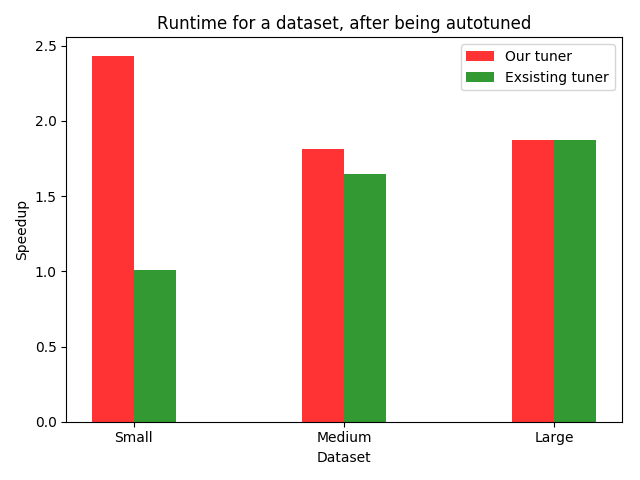
\includegraphics[width=.7\textwidth]{../benchmarks/LocVolCalibSML.png}
  \caption{The result for autotuning \textit{LocVolCalib} program, with no tuning being the baseline.}
	\label{LocVolCalib-SmallMediumLarge}
\end{figure}
In Figure \ref{LocVolCalib-SmallMediumLarge} we see that on all datasets the
threshold values our auto-tuner produced improved the performance of the
program. It's also clear that our auto-tuner found a set of values that made
the program perform better on \textit{small} and \textit{medium} than the
existing auto-tuner. The one problem, which cannot be seen in this graph is the
time it takes for each of the auto-tuners to tune the program. For the existing
auto-tuner it took around 17 minutes, whereas for our auto-tuner it took a
little under 23 hours, which is obviously far to slow to be of use in almost
all cases. 

%It is important to note, that \textit{large} is about XXX larger than \textit{medium}, while \textit{medium} is only XXX larger than \textit{small}
